\chapter{Aberrations of the Eye}

Most of the report will be devoted to correcting the first two types of aberrations, myopia, or nearsightedness, and hyperopia, or farsightedness. These two types of aberrations are examples of defocus, where the user focuses at a distance different from the that of the object, and are easiest to illustrate via a Gaussian ray tracing model. They are by far the most common aberrations and are the easiest to correct using a vision correcting display. We then go on to describe other types of aberrations such as astigmatism, coma, and trefoil, which are modeled using Zernike polynomials. Although these aberrations are much harder to correct, they represent a major subject of interest for future work.

\section{Gaussian Ray Tracing}

\begin{figure}[h!]
  \centering
  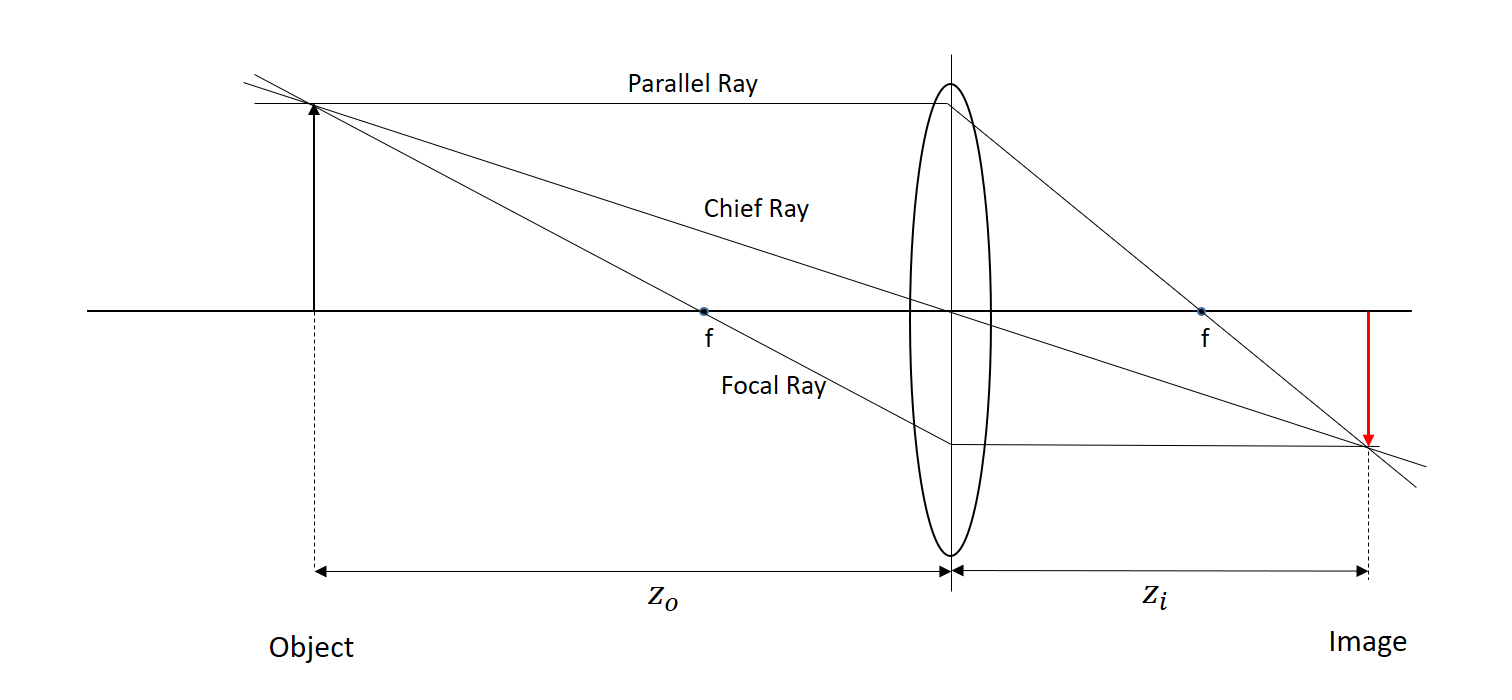
\includegraphics[width=5.0in]{chapters/chapter2/images/gauss.png}
  \caption{Gaussian Ray Tracing}
  \label{fig:gaussian}
\end{figure}

The Gaussian ray tracing model illustrates the path of light rays passing through an ideal thin lens. The lens contains a focal point where all of the light rays are focused, and the eye focuses at a focal plane. Three light rays are drawn: The parallel ray travels parallel to the viewing axis, and bends to the focal point behind the lens. The chief ray travels straight through the center of the lens without bending. The focal ray travels to the first focal point in front of the lens and bends parallel to the viewing axis after hitting the lens. An image is formed where the three rays intersect. In a perfect or ideal eye, the object is located at the focal plane, and the light rays traveling through the pupil converge on the sensor (retina on the eye).  The distance from the object to the lens ($z_o$) and the distance from the image to the lens ($z_i$) are related by the following equation: 

$$\frac{1}{f} = \frac{1}{z_i} + \frac{1}{z_o}$$
 
\section{Myopia}
In a myopic or nearsighted eye, the focal plane is in front of the object, and light rays converge in front of the retina. A myopic viewer does not have trouble seeing objects up close but cannot see objects far away. 

\begin{figure}[h!]
  \centering
  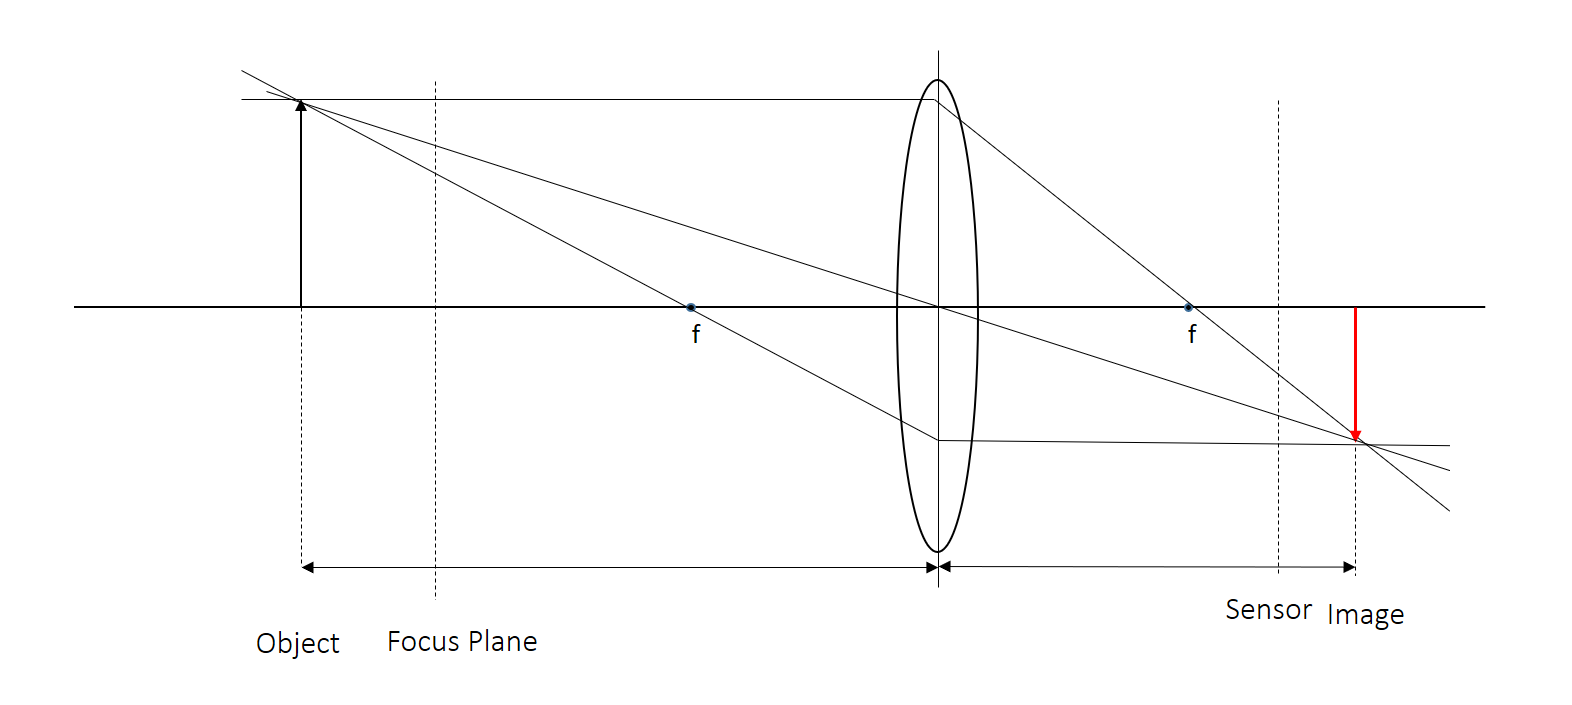
\includegraphics[width=5.0in]{chapters/chapter2/images/myopia.png}
  \caption{Myopia}
  \label{fig:myopia}
\end{figure}

Myopia affects about 30 to 40 percent among adults in Europe and the United States, and up to 80 percent or higher in the Asian population, especially in China \cite{allaboutvision:2016}. In addition, incidence of myopia is increasing, from about 25.0\% percent of Americans in 1971-1972 to 41.6\% in 1999-2004 \cite{Vitae:2009}.

% Cite this: http://www.allaboutvision.com/parents/myopia-progression.htm

\section{Hyperopia}
In a hyperopic or farsighted eye, light rays converge behind the retina. The viewer has a easier time from seeing far away, but an image that is close looks blurred. 

\begin{figure}[h!]
  \centering
  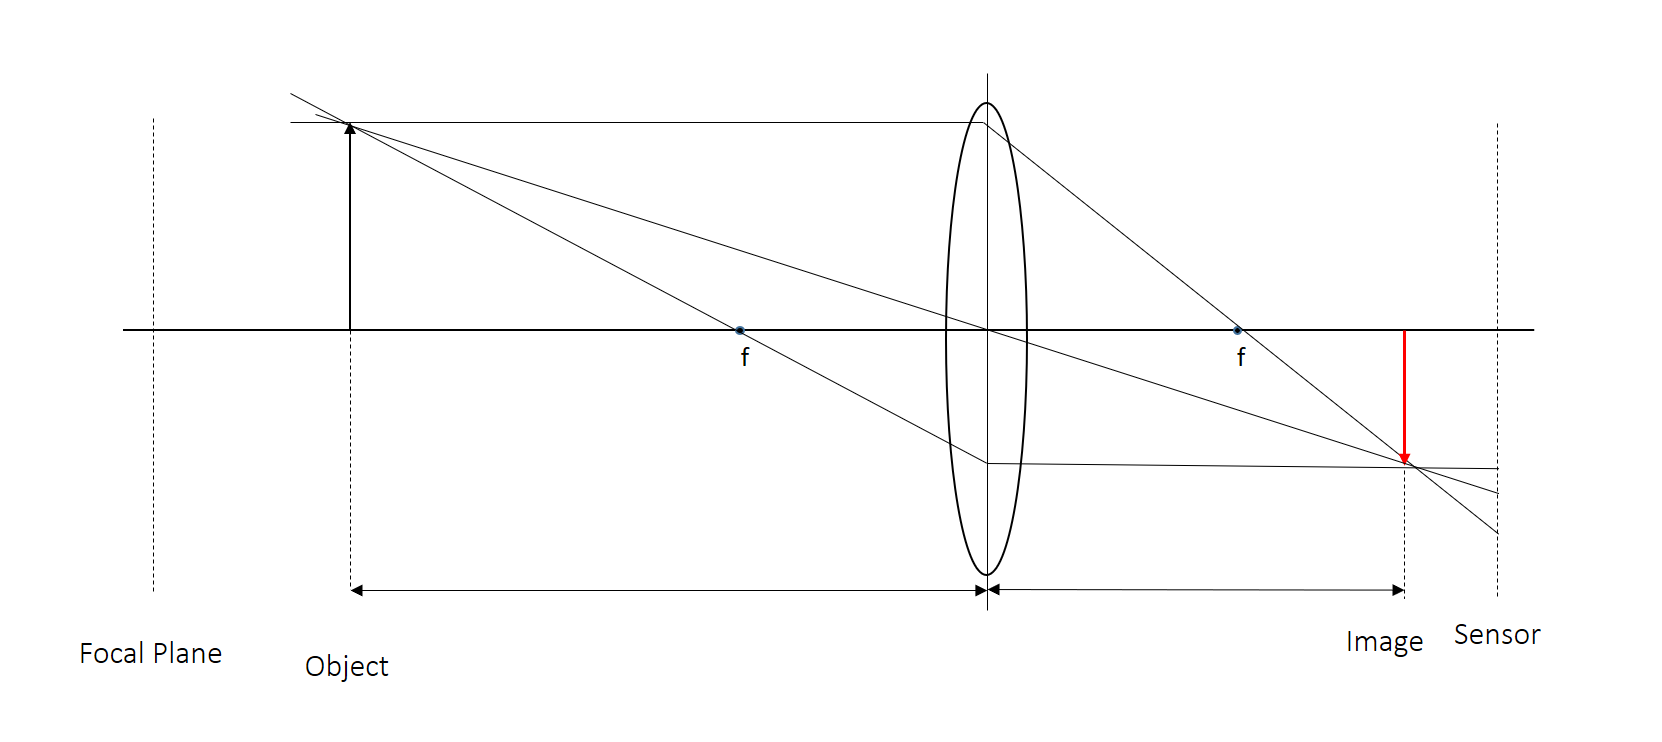
\includegraphics[width=5.0in]{chapters/chapter2/images/hyperopia.png}
  \caption{Hyperopia}
  \label{fig:hyperopia}
\end{figure}

Hyperopia is a common condition that affects about five to ten percent of the United States population \cite{NEI}. It can affect both children and adults, and people whose parents have hyperopia may also be more likely to get the condition.


\section{Zernike Polynomials and Higher Order Aberrations}

The pupil in the eye captures a wavefront, which is a surface in which the waves have a constant phase. The light rays are all perpendicular to the wavefront, and an aberrated wavefront is one in which not all of the rays traveling out of the wavefront surface travel through the same focal point. We fit the wave aberrations with the Zernike polynomials, which are a set of shapes orthogonal to the unit disk used to measure the eye’s wavefront \cite{Weisstein:Zernike}. The Zernike shapes are very similar to the usual aberrations that are found in a human eye. If we consider $W(x,y)$ as the wavefront, then here is the equation that fits the Zernike polynomial:

$$W(x,y)= \sum_{i} c_i Z_i (x,y)$$

$i$ represents the index of the coefficient $c$, and $Z(x,y)$ is the associated polynomial equation. Here are the first six terms of the Zernike polynomial:

\begin{equation}
\begin{aligned}
W(x,y) ={} & c_0 \times 1 + c_1 \times 2 \times \rho \times sin(\theta) + c_2 \times 2 \times \rho \times cos(\theta) \\
           & + c_3 \times \sqrt{6} \rho^2 \times sin(2\theta) + c_4 \times \sqrt{3} \times (2 \times \rho^2 - 1) \\
           & + c_5 \times \sqrt{6} \times \rho^2 \times cos(2\theta) + ...
\end{aligned}
\end{equation}

\begin{figure}[ht]
  \centering
  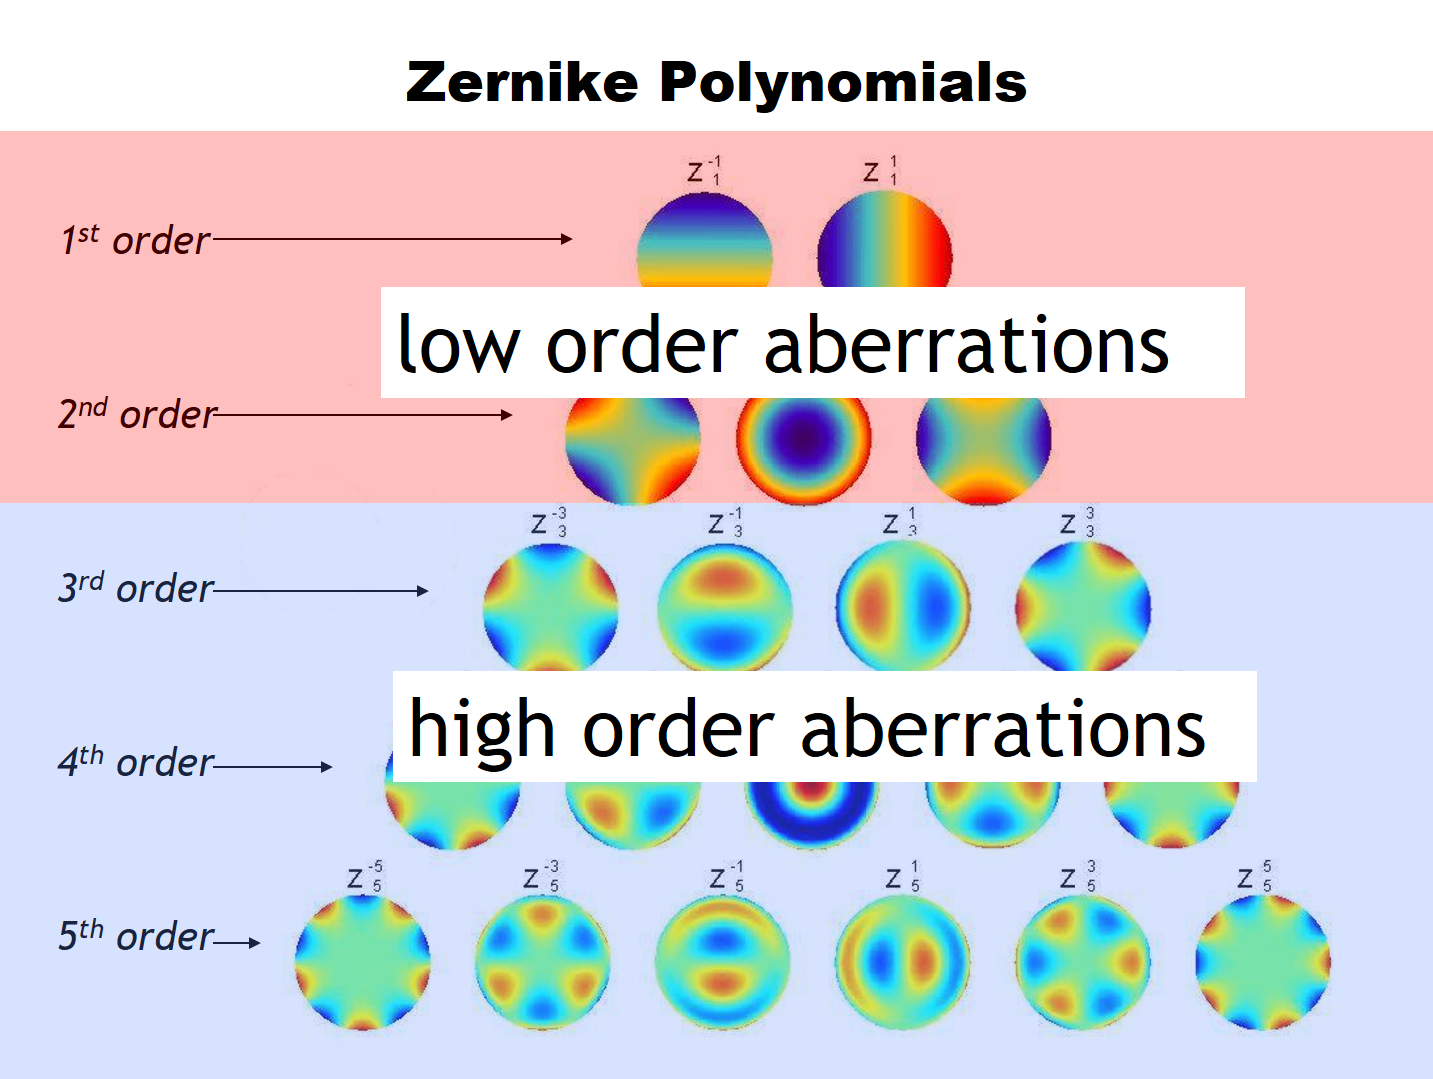
\includegraphics[width=5.0in]{chapters/chapter2/images/Zernike_polynomials.png}
  \caption{Zernike Polynomials \cite{Austin}}
  \label{fig:zernike}
\end{figure}

The first six Zernike polynomial terms measure lower order aberrations and the next sixty terms measure higher order aberrations. The names of lower order aberrations are tilt (terms one and two), astigmatism (terms three and five), and defocus (term four). Some examples of higher order aberrations are coma and trefoil (terms six through nine) and quatrefoil, secondary astigmatism, and spherical aberration (terms ten through fifteen). Lower order aberrations account for 90 percent of all decline in the quality of retinal images \cite{DIAS-SANTOS:2014}, while higher order aberrations account for the remaining 10 percent. Lower order aberrations are frequently treated with eyeglasses, which divert the direction of light rays so that they land squarely on the retina. However, higher order aberrations are much harder to treat with eyeglasses, but with the vision correction display, a user can input the Zernike polynomial coefficients to manipulate the image on the screen. 

% Cite this paper: http://www.scielo.br/pdf/rbof/v73n6/0034-7280-rbof-73-06-0358.pdf

% Question: Do I cite the PSF and wavefront map stuff?

% Do I mention circle of confusion?


% Cite Professor Austin's powerpoint slide

